\documentclass[tikz,border=6pt]{standalone}
\usepackage{amsmath}
\usetikzlibrary{arrows.meta,calc,patterns,positioning}
\begin{document}

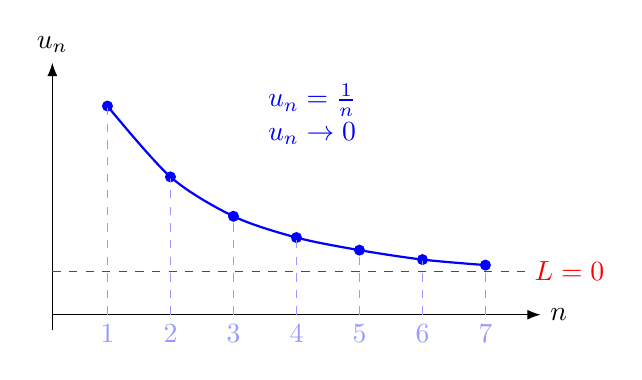
\begin{tikzpicture}[>=Latex,scale=1]
  \draw[->] (0,0) -- (6.2,0) node[right] {$n$};
  \draw[->] (0,-0.2) -- (0,3.2) node[above] {$u_n$};
  \draw[dashed,red] (0,0.55) -- (6,0.55) node[right] {$L=0$};
  \foreach \x/\y/\lab in {0.7/2.65/1,1.5/1.75/2,2.3/1.25/3,3.1/0.98/4,3.9/0.82/5,4.7/0.70/6,5.5/0.63/7} {
    \fill[blue] (\x,\y) circle (2pt);
    \draw[dashed,blue!40] (\x,0) node[below] {$\lab$} -- (\x,\y);
  }
  \draw[blue,thick] plot[smooth] coordinates {(0.7,2.65) (1.5,1.75) (2.3,1.25) (3.1,0.98) (3.9,0.82) (4.7,0.70) (5.5,0.63)};
  \node[align=left,blue] at (3.3,2.55) {$u_n=\frac{1}{n}$\\$u_n\to 0$};
\end{tikzpicture}

\end{document}
